\documentclass[1p]{elsarticle_modified}
%\bibliographystyle{elsarticle-num}

%\usepackage[colorlinks]{hyperref}
%\usepackage{abbrmath_seonhwa} %\Abb, \Ascr, \Acal ,\Abf, \Afrak
\usepackage{amsfonts}
\usepackage{amssymb}
\usepackage{amsmath}
\usepackage{amsthm}
\usepackage{scalefnt}
\usepackage{amsbsy}
\usepackage{kotex}
\usepackage{caption}
\usepackage{subfig}
\usepackage{color}
\usepackage{graphicx}
\usepackage{xcolor} %% white, black, red, green, blue, cyan, magenta, yellow
\usepackage{float}
\usepackage{setspace}
\usepackage{hyperref}

\usepackage{tikz}
\usetikzlibrary{arrows}

\usepackage{multirow}
\usepackage{array} % fixed length table
\usepackage{hhline}

%%%%%%%%%%%%%%%%%%%%%
\makeatletter
\renewcommand*\env@matrix[1][\arraystretch]{%
	\edef\arraystretch{#1}%
	\hskip -\arraycolsep
	\let\@ifnextchar\new@ifnextchar
	\array{*\c@MaxMatrixCols c}}
\makeatother %https://tex.stackexchange.com/questions/14071/how-can-i-increase-the-line-spacing-in-a-matrix
%%%%%%%%%%%%%%%

\usepackage[normalem]{ulem}

\newcommand{\msout}[1]{\ifmmode\text{\sout{\ensuremath{#1}}}\else\sout{#1}\fi}
%SOURCE: \msout is \stkout macro in https://tex.stackexchange.com/questions/20609/strikeout-in-math-mode

\newcommand{\cancel}[1]{
	\ifmmode
	{\color{red}\msout{#1}}
	\else
	{\color{red}\sout{#1}}
	\fi
}

\newcommand{\add}[1]{
	{\color{blue}\uwave{#1}}
}

\newcommand{\replace}[2]{
	\ifmmode
	{\color{red}\msout{#1}}{\color{blue}\uwave{#2}}
	\else
	{\color{red}\sout{#1}}{\color{blue}\uwave{#2}}
	\fi
}

\newcommand{\Sol}{\mathcal{S}} %segment
\newcommand{\D}{D} %diagram
\newcommand{\A}{\mathcal{A}} %arc


%%%%%%%%%%%%%%%%%%%%%%%%%%%%%5 test

\def\sl{\operatorname{\textup{SL}}(2,\Cbb)}
\def\psl{\operatorname{\textup{PSL}}(2,\Cbb)}
\def\quan{\mkern 1mu \triangleright \mkern 1mu}

\theoremstyle{definition}
\newtheorem{thm}{Theorem}[section]
\newtheorem{prop}[thm]{Proposition}
\newtheorem{lem}[thm]{Lemma}
\newtheorem{ques}[thm]{Question}
\newtheorem{cor}[thm]{Corollary}
\newtheorem{defn}[thm]{Definition}
\newtheorem{exam}[thm]{Example}
\newtheorem{rmk}[thm]{Remark}
\newtheorem{alg}[thm]{Algorithm}

\newcommand{\I}{\sqrt{-1}}
\begin{document}

%\begin{frontmatter}
%
%\title{Boundary parabolic representations of knots up to 8 crossings}
%
%%% Group authors per affiliation:
%\author{Yunhi Cho} 
%\address{Department of Mathematics, University of Seoul, Seoul, Korea}
%\ead{yhcho@uos.ac.kr}
%
%
%\author{Seonhwa Kim} %\fnref{s_kim}}
%\address{Center for Geometry and Physics, Institute for Basic Science, Pohang, 37673, Korea}
%\ead{ryeona17@ibs.re.kr}
%
%\author{Hyuk Kim}
%\address{Department of Mathematical Sciences, Seoul National University, Seoul 08826, Korea}
%\ead{hyukkim@snu.ac.kr}
%
%\author{Seokbeom Yoon}
%\address{Department of Mathematical Sciences, Seoul National University, Seoul, 08826,  Korea}
%\ead{sbyoon15@snu.ac.kr}
%
%\begin{abstract}
%We find all boundary parabolic representation of knots up to 8 crossings.
%
%\end{abstract}
%\begin{keyword}
%    \MSC[2010] 57M25 
%\end{keyword}
%
%\end{frontmatter}

%\linenumbers
%\tableofcontents
%
\newcommand\colored[1]{\textcolor{white}{\rule[-0.35ex]{0.8em}{1.4ex}}\kern-0.8em\color{red} #1}%
%\newcommand\colored[1]{\textcolor{white}{ #1}\kern-2.17ex	\textcolor{white}{ #1}\kern-1.81ex	\textcolor{white}{ #1}\kern-2.15ex\color{red}#1	}

{\Large $\underline{12n_{0874}~(K12n_{0874})}$}

\setlength{\tabcolsep}{10pt}
\renewcommand{\arraystretch}{1.6}
\vspace{1cm}\begin{tabular}{m{100pt}>{\centering\arraybackslash}m{274pt}}
\multirow{5}{120pt}{
	\centering
	\includegraphics[width=112pt]{../../../GIT/diagram.site/Diagrams/png/2963_12n_0874.png}\\
\ \ \ A knot diagram\footnotemark}&
\allowdisplaybreaks
\textbf{Linearized knot diagam} \\
\cline{2-2}
 &
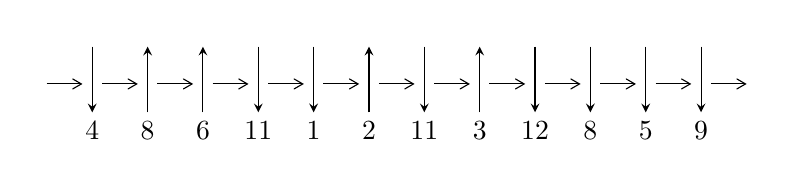
\begin{tikzpicture}[x=20pt, y=17pt]
	% nodes
	\node (C0) at (0, 0) {};
	\node (C1) at (1, 0) {};
	\node (C1U) at (1, +1) {};
	\node (C1D) at (1, -1) {4};

	\node (C2) at (2, 0) {};
	\node (C2U) at (2, +1) {};
	\node (C2D) at (2, -1) {8};

	\node (C3) at (3, 0) {};
	\node (C3U) at (3, +1) {};
	\node (C3D) at (3, -1) {6};

	\node (C4) at (4, 0) {};
	\node (C4U) at (4, +1) {};
	\node (C4D) at (4, -1) {11};

	\node (C5) at (5, 0) {};
	\node (C5U) at (5, +1) {};
	\node (C5D) at (5, -1) {1};

	\node (C6) at (6, 0) {};
	\node (C6U) at (6, +1) {};
	\node (C6D) at (6, -1) {2};

	\node (C7) at (7, 0) {};
	\node (C7U) at (7, +1) {};
	\node (C7D) at (7, -1) {11};

	\node (C8) at (8, 0) {};
	\node (C8U) at (8, +1) {};
	\node (C8D) at (8, -1) {3};

	\node (C9) at (9, 0) {};
	\node (C9U) at (9, +1) {};
	\node (C9D) at (9, -1) {12};

	\node (C10) at (10, 0) {};
	\node (C10U) at (10, +1) {};
	\node (C10D) at (10, -1) {8};

	\node (C11) at (11, 0) {};
	\node (C11U) at (11, +1) {};
	\node (C11D) at (11, -1) {5};

	\node (C12) at (12, 0) {};
	\node (C12U) at (12, +1) {};
	\node (C12D) at (12, -1) {9};
	\node (C13) at (13, 0) {};

	% arrows
	\draw[->,>={angle 60}]
	(C0) edge (C1) (C1) edge (C2) (C2) edge (C3) (C3) edge (C4) (C4) edge (C5) (C5) edge (C6) (C6) edge (C7) (C7) edge (C8) (C8) edge (C9) (C9) edge (C10) (C10) edge (C11) (C11) edge (C12) (C12) edge (C13) ;	\draw[->,>=stealth]
	(C1U) edge (C1D) (C2D) edge (C2U) (C3D) edge (C3U) (C4U) edge (C4D) (C5U) edge (C5D) (C6D) edge (C6U) (C7U) edge (C7D) (C8D) edge (C8U) (C9U) edge (C9D) (C10U) edge (C10D) (C11U) edge (C11D) (C12U) edge (C12D) ;
	\end{tikzpicture} \\
\hhline{~~} \\& 
\textbf{Solving Sequence} \\ \cline{2-2} 
 &
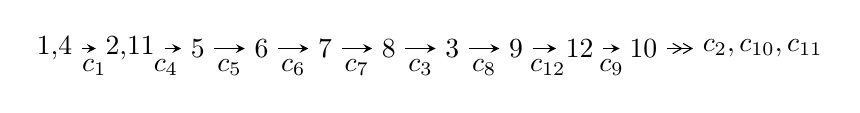
\begin{tikzpicture}[x=23pt, y=7pt]
	% node
	\node (A0) at (-1/8, 0) {1,4};
	\node (A1) at (17/16, 0) {2,11};
	\node (A2) at (17/8, 0) {5};
	\node (A3) at (25/8, 0) {6};
	\node (A4) at (33/8, 0) {7};
	\node (A5) at (41/8, 0) {8};
	\node (A6) at (49/8, 0) {3};
	\node (A7) at (57/8, 0) {9};
	\node (A8) at (65/8, 0) {12};
	\node (A9) at (73/8, 0) {10};
	\node (C1) at (1/2, -1) {$c_{1}$};
	\node (C2) at (13/8, -1) {$c_{4}$};
	\node (C3) at (21/8, -1) {$c_{5}$};
	\node (C4) at (29/8, -1) {$c_{6}$};
	\node (C5) at (37/8, -1) {$c_{7}$};
	\node (C6) at (45/8, -1) {$c_{3}$};
	\node (C7) at (53/8, -1) {$c_{8}$};
	\node (C8) at (61/8, -1) {$c_{12}$};
	\node (C9) at (69/8, -1) {$c_{9}$};
	\node (A10) at (11, 0) {$c_{2},c_{10},c_{11}$};

	% edge
	\draw[->,>=stealth]	
	(A0) edge (A1) (A1) edge (A2) (A2) edge (A3) (A3) edge (A4) (A4) edge (A5) (A5) edge (A6) (A6) edge (A7) (A7) edge (A8) (A8) edge (A9) ;
	\draw[->>,>={angle 60}]	
	(A9) edge (A10);
\end{tikzpicture} \\ 

\end{tabular} \\

\footnotetext{
The image of knot diagram is generated by the software ``\textbf{Draw programme}" developed by Andrew Bartholomew(\url{http://www.layer8.co.uk/maths/draw/index.htm\#Running-draw}), where we modified some parts for our purpose(\url{https://github.com/CATsTAILs/LinksPainter}).
}\phantom \\ \newline 
\centering \textbf{Ideals for irreducible components\footnotemark of $X_{\text{par}}$} 
 
\begin{align*}
I^u_{1}&=\langle 
3.88703\times10^{531} u^{97}+2.37179\times10^{532} u^{96}+\cdots+7.13036\times10^{532} b+1.66917\times10^{536},\\
\phantom{I^u_{1}}&\phantom{= \langle  }-5.17946\times10^{536} u^{97}-3.44558\times10^{537} u^{96}+\cdots+1.04681\times10^{537} a-6.30093\times10^{541},\\
\phantom{I^u_{1}}&\phantom{= \langle  }u^{98}+7 u^{97}+\cdots+485513 u+44043\rangle \\
I^u_{2}&=\langle 
-3.11544\times10^{51} u^{35}-1.76100\times10^{52} u^{34}+\cdots+5.72391\times10^{50} b-4.79348\times10^{51},\\
\phantom{I^u_{2}}&\phantom{= \langle  }-8.61463\times10^{50} u^{35}-4.68417\times10^{51} u^{34}+\cdots+5.72391\times10^{50} a-8.17523\times10^{50},\;u^{36}+5 u^{35}+\cdots+5 u-1\rangle \\
I^u_{3}&=\langle 
b+a-1,\;a^2- a+1,\;u-1\rangle \\
I^u_{4}&=\langle 
b+2,\;a+1,\;u+1\rangle \\
\\
\end{align*}
\raggedright * 4 irreducible components of $\dim_{\mathbb{C}}=0$, with total 137 representations.\\
\footnotetext{All coefficients of polynomials are rational numbers. But the coefficients are sometimes approximated in decimal forms when there is not enough margin.}
\newpage
\renewcommand{\arraystretch}{1}
\centering \section*{I. $I^u_{1}= \langle 3.89\times10^{531} u^{97}+2.37\times10^{532} u^{96}+\cdots+7.13\times10^{532} b+1.67\times10^{536},\;-5.18\times10^{536} u^{97}-3.45\times10^{537} u^{96}+\cdots+1.05\times10^{537} a-6.30\times10^{541},\;u^{98}+7 u^{97}+\cdots+485513 u+44043 \rangle$}
\flushleft \textbf{(i) Arc colorings}\\
\begin{tabular}{m{7pt} m{180pt} m{7pt} m{180pt} }
\flushright $a_{1}=$&$\begin{pmatrix}1\\0\end{pmatrix}$ \\
\flushright $a_{4}=$&$\begin{pmatrix}0\\u\end{pmatrix}$ \\
\flushright $a_{2}=$&$\begin{pmatrix}1\\u^2\end{pmatrix}$ \\
\flushright $a_{11}=$&$\begin{pmatrix}0.494786 u^{97}+3.29152 u^{96}+\cdots+498696. u+60191.9\\-0.0545138 u^{97}-0.332633 u^{96}+\cdots-23823.2 u-2340.93\end{pmatrix}$ \\
\flushright $a_{5}=$&$\begin{pmatrix}0.290645 u^{97}+1.90277 u^{96}+\cdots+246755. u+28003.6\\0.0713382 u^{97}+0.477526 u^{96}+\cdots+70483.3 u+8186.59\end{pmatrix}$ \\
\flushright $a_{6}=$&$\begin{pmatrix}0.219307 u^{97}+1.42524 u^{96}+\cdots+176271. u+19817.0\\0.0713382 u^{97}+0.477526 u^{96}+\cdots+70483.3 u+8186.59\end{pmatrix}$ \\
\flushright $a_{7}=$&$\begin{pmatrix}0.234515 u^{97}+1.53885 u^{96}+\cdots+203052. u+23162.9\\0.0576709 u^{97}+0.395768 u^{96}+\cdots+66339.8 u+7871.48\end{pmatrix}$ \\
\flushright $a_{8}=$&$\begin{pmatrix}0.663198 u^{97}+4.31867 u^{96}+\cdots+548562. u+62433.4\\0.187423 u^{97}+1.21229 u^{96}+\cdots+146315. u+16359.9\end{pmatrix}$ \\
\flushright $a_{3}=$&$\begin{pmatrix}-0.452513 u^{97}-2.97505 u^{96}+\cdots-412430. u-48480.8\\-0.0874361 u^{97}-0.577292 u^{96}+\cdots-82676.3 u-9809.37\end{pmatrix}$ \\
\flushright $a_{9}=$&$\begin{pmatrix}0.258820 u^{97}+1.64422 u^{96}+\cdots+157464. u+15829.2\\0.134219 u^{97}+0.851277 u^{96}+\cdots+80780.0 u+7907.17\end{pmatrix}$ \\
\flushright $a_{12}=$&$\begin{pmatrix}1.60879 u^{97}+10.6591 u^{96}+\cdots+1.59375\times10^{6} u+192950.\\0.0194880 u^{97}+0.128613 u^{96}+\cdots+19715.0 u+2307.08\end{pmatrix}$ \\
\flushright $a_{10}=$&$\begin{pmatrix}0.815945 u^{97}+5.34673 u^{96}+\cdots+737122. u+86857.8\\0.186275 u^{97}+1.16701 u^{96}+\cdots+108090. u+11163.4\end{pmatrix}$\\&\end{tabular}
\flushleft \textbf{(ii) Obstruction class $= -1$}\\~\\
\flushleft \textbf{(iii) Cusp Shapes $= 1.36407 u^{97}+8.16421 u^{96}+\cdots+290793. u+4941.92$}\\~\\
\newpage\renewcommand{\arraystretch}{1}
\flushleft \textbf{(iv) u-Polynomials at the component}\newline \\
\begin{tabular}{m{50pt}|m{274pt}}
Crossings & \hspace{64pt}u-Polynomials at each crossing \\
\hline $$\begin{aligned}c_{1}\end{aligned}$$&$\begin{aligned}
&u^{98}-7 u^{97}+\cdots-485513 u+44043
\end{aligned}$\\
\hline $$\begin{aligned}c_{2},c_{8}\end{aligned}$$&$\begin{aligned}
&u^{98}-21 u^{96}+\cdots+16624 u+2701
\end{aligned}$\\
\hline $$\begin{aligned}c_{3}\end{aligned}$$&$\begin{aligned}
&u^{98}+5 u^{97}+\cdots-60 u-3
\end{aligned}$\\
\hline $$\begin{aligned}c_{4},c_{11}\end{aligned}$$&$\begin{aligned}
&u^{98}-3 u^{97}+\cdots-1324 u-193
\end{aligned}$\\
\hline $$\begin{aligned}c_{5}\end{aligned}$$&$\begin{aligned}
&u^{98}+4 u^{97}+\cdots+9488 u+1852
\end{aligned}$\\
\hline $$\begin{aligned}c_{6}\end{aligned}$$&$\begin{aligned}
&u^{98}+28 u^{96}+\cdots+1451470765 u-470778887
\end{aligned}$\\
\hline $$\begin{aligned}c_{7},c_{10}\end{aligned}$$&$\begin{aligned}
&u^{98}-5 u^{97}+\cdots+7560885 u-625281
\end{aligned}$\\
\hline $$\begin{aligned}c_{9},c_{12}\end{aligned}$$&$\begin{aligned}
&u^{98}-6 u^{97}+\cdots-11140 u+837
\end{aligned}$\\
\hline
\end{tabular}\\~\\
\newpage\renewcommand{\arraystretch}{1}
\flushleft \textbf{(v) Riley Polynomials at the component}\newline \\
\begin{tabular}{m{50pt}|m{274pt}}
Crossings & \hspace{64pt}Riley Polynomials at each crossing \\
\hline $$\begin{aligned}c_{1}\end{aligned}$$&$\begin{aligned}
&y^{98}-51 y^{97}+\cdots-123544471309 y+1939785849
\end{aligned}$\\
\hline $$\begin{aligned}c_{2},c_{8}\end{aligned}$$&$\begin{aligned}
&y^{98}-42 y^{97}+\cdots-258320098 y+7295401
\end{aligned}$\\
\hline $$\begin{aligned}c_{3}\end{aligned}$$&$\begin{aligned}
&y^{98}-5 y^{97}+\cdots-822 y+9
\end{aligned}$\\
\hline $$\begin{aligned}c_{4},c_{11}\end{aligned}$$&$\begin{aligned}
&y^{98}-73 y^{97}+\cdots-1306760 y+37249
\end{aligned}$\\
\hline $$\begin{aligned}c_{5}\end{aligned}$$&$\begin{aligned}
&y^{98}-24 y^{97}+\cdots-12001088 y+3429904
\end{aligned}$\\
\hline $$\begin{aligned}c_{6}\end{aligned}$$&$\begin{aligned}
&y^{98}+56 y^{97}+\cdots+1.14\times10^{19} y+2.22\times10^{17}
\end{aligned}$\\
\hline $$\begin{aligned}c_{7},c_{10}\end{aligned}$$&$\begin{aligned}
&y^{98}-89 y^{97}+\cdots-6238806215403 y+390976328961
\end{aligned}$\\
\hline $$\begin{aligned}c_{9},c_{12}\end{aligned}$$&$\begin{aligned}
&y^{98}+28 y^{97}+\cdots+524678 y+700569
\end{aligned}$\\
\hline
\end{tabular}\\~\\
\newpage\flushleft \textbf{(vi) Complex Volumes and Cusp Shapes}
$$\begin{array}{c|c|c}  
\text{Solutions to }I^u_{1}& \I (\text{vol} + \sqrt{-1}CS) & \text{Cusp shape}\\
 \hline 
\begin{aligned}
u &= \phantom{-}0.968126 + 0.222153 I \\
a &= -0.49504 - 1.35651 I \\
b &= \phantom{-}0.081167 + 0.136365 I\end{aligned}
 & -2.30647 - 3.35687 I & \phantom{-0.000000 } 0 \\ \hline\begin{aligned}
u &= \phantom{-}0.968126 - 0.222153 I \\
a &= -0.49504 + 1.35651 I \\
b &= \phantom{-}0.081167 - 0.136365 I\end{aligned}
 & -2.30647 + 3.35687 I & \phantom{-0.000000 } 0 \\ \hline\begin{aligned}
u &= \phantom{-}0.946901 + 0.283855 I \\
a &= \phantom{-}0.833414 + 1.130270 I \\
b &= \phantom{-}0.151296 - 0.072870 I\end{aligned}
 & -2.46721 + 1.31247 I & \phantom{-0.000000 } 0 \\ \hline\begin{aligned}
u &= \phantom{-}0.946901 - 0.283855 I \\
a &= \phantom{-}0.833414 - 1.130270 I \\
b &= \phantom{-}0.151296 + 0.072870 I\end{aligned}
 & -2.46721 - 1.31247 I & \phantom{-0.000000 } 0 \\ \hline\begin{aligned}
u &= -0.920116 + 0.440938 I \\
a &= -1.47718 - 0.39312 I \\
b &= -1.67990 + 0.45771 I\end{aligned}
 & -1.08524 + 3.10232 I & \phantom{-0.000000 } 0 \\ \hline\begin{aligned}
u &= -0.920116 - 0.440938 I \\
a &= -1.47718 + 0.39312 I \\
b &= -1.67990 - 0.45771 I\end{aligned}
 & -1.08524 - 3.10232 I & \phantom{-0.000000 } 0 \\ \hline\begin{aligned}
u &= \phantom{-}0.801784 + 0.518175 I \\
a &= \phantom{-}1.105210 - 0.820593 I \\
b &= \phantom{-}1.50280 - 1.10221 I\end{aligned}
 & -5.09430 + 4.73289 I & \phantom{-0.000000 } 0 \\ \hline\begin{aligned}
u &= \phantom{-}0.801784 - 0.518175 I \\
a &= \phantom{-}1.105210 + 0.820593 I \\
b &= \phantom{-}1.50280 + 1.10221 I\end{aligned}
 & -5.09430 - 4.73289 I & \phantom{-0.000000 } 0 \\ \hline\begin{aligned}
u &= \phantom{-}0.897499 + 0.319102 I \\
a &= -0.772552 + 0.279139 I \\
b &= -1.94191 - 1.28646 I\end{aligned}
 & -3.55756 - 2.03098 I & \phantom{-0.000000 } 0 \\ \hline\begin{aligned}
u &= \phantom{-}0.897499 - 0.319102 I \\
a &= -0.772552 - 0.279139 I \\
b &= -1.94191 + 1.28646 I\end{aligned}
 & -3.55756 + 2.03098 I & \phantom{-0.000000 } 0\\
 \hline 
 \end{array}$$\newpage$$\begin{array}{c|c|c}  
\text{Solutions to }I^u_{1}& \I (\text{vol} + \sqrt{-1}CS) & \text{Cusp shape}\\
 \hline 
\begin{aligned}
u &= -0.930790 + 0.500586 I \\
a &= \phantom{-}1.177720 + 0.296086 I \\
b &= \phantom{-}1.27067 + 0.69461 I\end{aligned}
 & -8.59494 + 1.86844 I & \phantom{-0.000000 } 0 \\ \hline\begin{aligned}
u &= -0.930790 - 0.500586 I \\
a &= \phantom{-}1.177720 - 0.296086 I \\
b &= \phantom{-}1.27067 - 0.69461 I\end{aligned}
 & -8.59494 - 1.86844 I & \phantom{-0.000000 } 0 \\ \hline\begin{aligned}
u &= \phantom{-}0.032690 + 1.075740 I \\
a &= -0.146955 + 0.681838 I \\
b &= \phantom{-}0.780704 + 0.134721 I\end{aligned}
 & \phantom{-}2.45073 - 4.36839 I & \phantom{-0.000000 } 0 \\ \hline\begin{aligned}
u &= \phantom{-}0.032690 - 1.075740 I \\
a &= -0.146955 - 0.681838 I \\
b &= \phantom{-}0.780704 - 0.134721 I\end{aligned}
 & \phantom{-}2.45073 + 4.36839 I & \phantom{-0.000000 } 0 \\ \hline\begin{aligned}
u &= \phantom{-}0.933459 + 0.540835 I \\
a &= \phantom{-}0.030560 - 0.426960 I \\
b &= \phantom{-}0.115481 + 1.261990 I\end{aligned}
 & -1.93431 + 1.15400 I & \phantom{-0.000000 } 0 \\ \hline\begin{aligned}
u &= \phantom{-}0.933459 - 0.540835 I \\
a &= \phantom{-}0.030560 + 0.426960 I \\
b &= \phantom{-}0.115481 - 1.261990 I\end{aligned}
 & -1.93431 - 1.15400 I & \phantom{-0.000000 } 0 \\ \hline\begin{aligned}
u &= -0.996957 + 0.439724 I \\
a &= \phantom{-}1.41379 + 0.09061 I \\
b &= \phantom{-}1.271260 + 0.256458 I\end{aligned}
 & -8.93133 + 2.06464 I & \phantom{-0.000000 } 0 \\ \hline\begin{aligned}
u &= -0.996957 - 0.439724 I \\
a &= \phantom{-}1.41379 - 0.09061 I \\
b &= \phantom{-}1.271260 - 0.256458 I\end{aligned}
 & -8.93133 - 2.06464 I & \phantom{-0.000000 } 0 \\ \hline\begin{aligned}
u &= \phantom{-}0.432657 + 1.007900 I \\
a &= \phantom{-}0.113369 - 0.588730 I \\
b &= \phantom{-}0.021279 - 0.650648 I\end{aligned}
 & \phantom{-}2.23861 - 1.82364 I & \phantom{-0.000000 } 0 \\ \hline\begin{aligned}
u &= \phantom{-}0.432657 - 1.007900 I \\
a &= \phantom{-}0.113369 + 0.588730 I \\
b &= \phantom{-}0.021279 + 0.650648 I\end{aligned}
 & \phantom{-}2.23861 + 1.82364 I & \phantom{-0.000000 } 0\\
 \hline 
 \end{array}$$\newpage$$\begin{array}{c|c|c}  
\text{Solutions to }I^u_{1}& \I (\text{vol} + \sqrt{-1}CS) & \text{Cusp shape}\\
 \hline 
\begin{aligned}
u &= -1.10330\phantom{ +0.000000I} \\
a &= -1.11211\phantom{ +0.000000I} \\
b &= -2.15012\phantom{ +0.000000I}\end{aligned}
 & -1.74309\phantom{ +0.000000I} & \phantom{-0.000000 } 0 \\ \hline\begin{aligned}
u &= \phantom{-}0.584477 + 0.938415 I \\
a &= \phantom{-}0.943522 - 0.377784 I \\
b &= \phantom{-}2.48816 + 0.38109 I\end{aligned}
 & \phantom{-}2.08534 - 8.07440 I & \phantom{-0.000000 } 0 \\ \hline\begin{aligned}
u &= \phantom{-}0.584477 - 0.938415 I \\
a &= \phantom{-}0.943522 + 0.377784 I \\
b &= \phantom{-}2.48816 - 0.38109 I\end{aligned}
 & \phantom{-}2.08534 + 8.07440 I & \phantom{-0.000000 } 0 \\ \hline\begin{aligned}
u &= -0.562422 + 0.961350 I \\
a &= -0.273104 - 0.316163 I \\
b &= -1.14512 + 1.43575 I\end{aligned}
 & -2.03759 + 0.63611 I & \phantom{-0.000000 } 0 \\ \hline\begin{aligned}
u &= -0.562422 - 0.961350 I \\
a &= -0.273104 + 0.316163 I \\
b &= -1.14512 - 1.43575 I\end{aligned}
 & -2.03759 - 0.63611 I & \phantom{-0.000000 } 0 \\ \hline\begin{aligned}
u &= -0.735376 + 0.852023 I \\
a &= -0.251086 + 1.031980 I \\
b &= \phantom{-}0.245412 + 0.151108 I\end{aligned}
 & \phantom{-}4.58637 - 0.17416 I & \phantom{-0.000000 } 0 \\ \hline\begin{aligned}
u &= -0.735376 - 0.852023 I \\
a &= -0.251086 - 1.031980 I \\
b &= \phantom{-}0.245412 - 0.151108 I\end{aligned}
 & \phantom{-}4.58637 + 0.17416 I & \phantom{-0.000000 } 0 \\ \hline\begin{aligned}
u &= \phantom{-}1.063820 + 0.379249 I \\
a &= \phantom{-}0.876645 + 0.506504 I \\
b &= \phantom{-}0.888153 - 0.336155 I\end{aligned}
 & -0.53158 - 2.92126 I & \phantom{-0.000000 } 0 \\ \hline\begin{aligned}
u &= \phantom{-}1.063820 - 0.379249 I \\
a &= \phantom{-}0.876645 - 0.506504 I \\
b &= \phantom{-}0.888153 + 0.336155 I\end{aligned}
 & -0.53158 + 2.92126 I & \phantom{-0.000000 } 0 \\ \hline\begin{aligned}
u &= \phantom{-}0.851429 + 0.099909 I \\
a &= \phantom{-}1.265410 - 0.154215 I \\
b &= \phantom{-}1.42389 + 1.17660 I\end{aligned}
 & \phantom{-}0.75470 - 2.36582 I & \phantom{-0.000000 } 0\\
 \hline 
 \end{array}$$\newpage$$\begin{array}{c|c|c}  
\text{Solutions to }I^u_{1}& \I (\text{vol} + \sqrt{-1}CS) & \text{Cusp shape}\\
 \hline 
\begin{aligned}
u &= \phantom{-}0.851429 - 0.099909 I \\
a &= \phantom{-}1.265410 + 0.154215 I \\
b &= \phantom{-}1.42389 - 1.17660 I\end{aligned}
 & \phantom{-}0.75470 + 2.36582 I & \phantom{-0.000000 } 0 \\ \hline\begin{aligned}
u &= -1.029330 + 0.506262 I \\
a &= \phantom{-}0.363470 - 1.016050 I \\
b &= -0.227694 - 0.002893 I\end{aligned}
 & -3.72389 + 3.86913 I & \phantom{-0.000000 } 0 \\ \hline\begin{aligned}
u &= -1.029330 - 0.506262 I \\
a &= \phantom{-}0.363470 + 1.016050 I \\
b &= -0.227694 + 0.002893 I\end{aligned}
 & -3.72389 - 3.86913 I & \phantom{-0.000000 } 0 \\ \hline\begin{aligned}
u &= -0.595068 + 0.597381 I \\
a &= -1.27394 - 1.13856 I \\
b &= -1.67648 - 1.21810 I\end{aligned}
 & -4.91130 + 7.00164 I & \phantom{-0.000000 } 0 \\ \hline\begin{aligned}
u &= -0.595068 - 0.597381 I \\
a &= -1.27394 + 1.13856 I \\
b &= -1.67648 + 1.21810 I\end{aligned}
 & -4.91130 - 7.00164 I & \phantom{-0.000000 } 0 \\ \hline\begin{aligned}
u &= \phantom{-}0.782994 + 0.856661 I \\
a &= -0.701326 + 0.841550 I \\
b &= -1.105620 + 0.657033 I\end{aligned}
 & -5.86798 - 2.06115 I & \phantom{-0.000000 } 0 \\ \hline\begin{aligned}
u &= \phantom{-}0.782994 - 0.856661 I \\
a &= -0.701326 - 0.841550 I \\
b &= -1.105620 - 0.657033 I\end{aligned}
 & -5.86798 + 2.06115 I & \phantom{-0.000000 } 0 \\ \hline\begin{aligned}
u &= \phantom{-}0.690803 + 0.464994 I \\
a &= \phantom{-}0.297748 - 0.174526 I \\
b &= \phantom{-}0.14837 - 1.74686 I\end{aligned}
 & -1.39771 - 4.15360 I & \phantom{-0.000000 } 0 \\ \hline\begin{aligned}
u &= \phantom{-}0.690803 - 0.464994 I \\
a &= \phantom{-}0.297748 + 0.174526 I \\
b &= \phantom{-}0.14837 + 1.74686 I\end{aligned}
 & -1.39771 + 4.15360 I & \phantom{-0.000000 } 0 \\ \hline\begin{aligned}
u &= \phantom{-}1.009410 + 0.601914 I \\
a &= \phantom{-}1.45556 - 0.07995 I \\
b &= \phantom{-}1.256130 + 0.160658 I\end{aligned}
 & -5.76243 - 9.39036 I & \phantom{-0.000000 } 0\\
 \hline 
 \end{array}$$\newpage$$\begin{array}{c|c|c}  
\text{Solutions to }I^u_{1}& \I (\text{vol} + \sqrt{-1}CS) & \text{Cusp shape}\\
 \hline 
\begin{aligned}
u &= \phantom{-}1.009410 - 0.601914 I \\
a &= \phantom{-}1.45556 + 0.07995 I \\
b &= \phantom{-}1.256130 - 0.160658 I\end{aligned}
 & -5.76243 + 9.39036 I & \phantom{-0.000000 } 0 \\ \hline\begin{aligned}
u &= -0.680166 + 0.457476 I \\
a &= \phantom{-}0.211622 - 0.117266 I \\
b &= \phantom{-}1.02928 - 2.02906 I\end{aligned}
 & \phantom{-}0.57382 - 6.84957 I & \phantom{-0.000000 } 0 \\ \hline\begin{aligned}
u &= -0.680166 - 0.457476 I \\
a &= \phantom{-}0.211622 + 0.117266 I \\
b &= \phantom{-}1.02928 + 2.02906 I\end{aligned}
 & \phantom{-}0.57382 + 6.84957 I & \phantom{-0.000000 } 0 \\ \hline\begin{aligned}
u &= \phantom{-}1.076280 + 0.493384 I \\
a &= -0.847870 + 0.513350 I \\
b &= -1.57841 - 0.74164 I\end{aligned}
 & -3.94589 - 2.30114 I & \phantom{-0.000000 } 0 \\ \hline\begin{aligned}
u &= \phantom{-}1.076280 - 0.493384 I \\
a &= -0.847870 - 0.513350 I \\
b &= -1.57841 + 0.74164 I\end{aligned}
 & -3.94589 + 2.30114 I & \phantom{-0.000000 } 0 \\ \hline\begin{aligned}
u &= -1.123600 + 0.379256 I \\
a &= -1.53393 - 0.07531 I \\
b &= -1.44831 + 0.00070 I\end{aligned}
 & -7.00593 - 2.93592 I & \phantom{-0.000000 } 0 \\ \hline\begin{aligned}
u &= -1.123600 - 0.379256 I \\
a &= -1.53393 + 0.07531 I \\
b &= -1.44831 - 0.00070 I\end{aligned}
 & -7.00593 + 2.93592 I & \phantom{-0.000000 } 0 \\ \hline\begin{aligned}
u &= -1.084890 + 0.492363 I \\
a &= -0.504486 + 1.158190 I \\
b &= \phantom{-}0.0828795 + 0.0778496 I\end{aligned}
 & -1.06566 + 10.79880 I & \phantom{-0.000000 } 0 \\ \hline\begin{aligned}
u &= -1.084890 - 0.492363 I \\
a &= -0.504486 - 1.158190 I \\
b &= \phantom{-}0.0828795 - 0.0778496 I\end{aligned}
 & -1.06566 - 10.79880 I & \phantom{-0.000000 } 0 \\ \hline\begin{aligned}
u &= -1.124510 + 0.448253 I \\
a &= \phantom{-}1.209100 + 0.200099 I \\
b &= \phantom{-}1.85028 - 0.67299 I\end{aligned}
 & -1.21930 + 8.61712 I & \phantom{-0.000000 } 0\\
 \hline 
 \end{array}$$\newpage$$\begin{array}{c|c|c}  
\text{Solutions to }I^u_{1}& \I (\text{vol} + \sqrt{-1}CS) & \text{Cusp shape}\\
 \hline 
\begin{aligned}
u &= -1.124510 - 0.448253 I \\
a &= \phantom{-}1.209100 - 0.200099 I \\
b &= \phantom{-}1.85028 + 0.67299 I\end{aligned}
 & -1.21930 - 8.61712 I & \phantom{-0.000000 } 0 \\ \hline\begin{aligned}
u &= -0.464509 + 1.172000 I \\
a &= -0.053836 + 0.261001 I \\
b &= \phantom{-}0.621028 - 0.197974 I\end{aligned}
 & \phantom{-}6.76349 + 2.34241 I & \phantom{-0.000000 } 0 \\ \hline\begin{aligned}
u &= -0.464509 - 1.172000 I \\
a &= -0.053836 - 0.261001 I \\
b &= \phantom{-}0.621028 + 0.197974 I\end{aligned}
 & \phantom{-}6.76349 - 2.34241 I & \phantom{-0.000000 } 0 \\ \hline\begin{aligned}
u &= -0.739123\phantom{ +0.000000I} \\
a &= \phantom{-}2.25200\phantom{ +0.000000I} \\
b &= \phantom{-}2.54683\phantom{ +0.000000I}\end{aligned}
 & -9.95144\phantom{ +0.000000I} & -118.510\phantom{ +0.000000I} \\ \hline\begin{aligned}
u &= -0.731020\phantom{ +0.000000I} \\
a &= -1.22807\phantom{ +0.000000I} \\
b &= -1.63973\phantom{ +0.000000I}\end{aligned}
 & -1.67876\phantom{ +0.000000I} & \phantom{-0.000000 } 0 \\ \hline\begin{aligned}
u &= -0.708249 + 0.175453 I \\
a &= \phantom{-}0.538567 - 0.513506 I \\
b &= \phantom{-}0.137723 - 0.377292 I\end{aligned}
 & \phantom{-}2.40542 - 1.79703 I & \phantom{-0.000000 } 0 \\ \hline\begin{aligned}
u &= -0.708249 - 0.175453 I \\
a &= \phantom{-}0.538567 + 0.513506 I \\
b &= \phantom{-}0.137723 + 0.377292 I\end{aligned}
 & \phantom{-}2.40542 + 1.79703 I & \phantom{-0.000000 } 0 \\ \hline\begin{aligned}
u &= \phantom{-}0.589743 + 1.141430 I \\
a &= -0.233114 - 0.785124 I \\
b &= -0.331529 - 0.320158 I\end{aligned}
 & \phantom{-}2.51262 - 2.70362 I & \phantom{-0.000000 } 0 \\ \hline\begin{aligned}
u &= \phantom{-}0.589743 - 1.141430 I \\
a &= -0.233114 + 0.785124 I \\
b &= -0.331529 + 0.320158 I\end{aligned}
 & \phantom{-}2.51262 + 2.70362 I & \phantom{-0.000000 } 0 \\ \hline\begin{aligned}
u &= \phantom{-}0.391378 + 0.596073 I \\
a &= \phantom{-}0.640441 + 0.147713 I \\
b &= \phantom{-}0.161637 - 0.141028 I\end{aligned}
 & -0.015074 - 1.217060 I & \phantom{-0.000000 } 0\\
 \hline 
 \end{array}$$\newpage$$\begin{array}{c|c|c}  
\text{Solutions to }I^u_{1}& \I (\text{vol} + \sqrt{-1}CS) & \text{Cusp shape}\\
 \hline 
\begin{aligned}
u &= \phantom{-}0.391378 - 0.596073 I \\
a &= \phantom{-}0.640441 - 0.147713 I \\
b &= \phantom{-}0.161637 + 0.141028 I\end{aligned}
 & -0.015074 + 1.217060 I & \phantom{-0.000000 } 0 \\ \hline\begin{aligned}
u &= \phantom{-}1.104790 + 0.665459 I \\
a &= -1.206870 + 0.214393 I \\
b &= -1.43304 - 0.12209 I\end{aligned}
 & -7.05257 - 3.86875 I & \phantom{-0.000000 } 0 \\ \hline\begin{aligned}
u &= \phantom{-}1.104790 - 0.665459 I \\
a &= -1.206870 - 0.214393 I \\
b &= -1.43304 + 0.12209 I\end{aligned}
 & -7.05257 + 3.86875 I & \phantom{-0.000000 } 0 \\ \hline\begin{aligned}
u &= \phantom{-}1.281240 + 0.166858 I \\
a &= \phantom{-}0.859196 - 0.472227 I \\
b &= \phantom{-}1.292930 + 0.430670 I\end{aligned}
 & -1.82405 + 2.36704 I & \phantom{-0.000000 } 0 \\ \hline\begin{aligned}
u &= \phantom{-}1.281240 - 0.166858 I \\
a &= \phantom{-}0.859196 + 0.472227 I \\
b &= \phantom{-}1.292930 - 0.430670 I\end{aligned}
 & -1.82405 - 2.36704 I & \phantom{-0.000000 } 0 \\ \hline\begin{aligned}
u &= -0.447035 + 1.215850 I \\
a &= -0.179136 - 0.116619 I \\
b &= \phantom{-}0.047631 + 0.526670 I\end{aligned}
 & \phantom{-}5.34790 + 6.03017 I & \phantom{-0.000000 } 0 \\ \hline\begin{aligned}
u &= -0.447035 - 1.215850 I \\
a &= -0.179136 + 0.116619 I \\
b &= \phantom{-}0.047631 - 0.526670 I\end{aligned}
 & \phantom{-}5.34790 - 6.03017 I & \phantom{-0.000000 } 0 \\ \hline\begin{aligned}
u &= -1.053150 + 0.760738 I \\
a &= \phantom{-}0.974388 - 0.043306 I \\
b &= \phantom{-}2.04585 - 0.47947 I\end{aligned}
 & \phantom{-}3.59575 + 6.15631 I & \phantom{-0.000000 } 0 \\ \hline\begin{aligned}
u &= -1.053150 - 0.760738 I \\
a &= \phantom{-}0.974388 + 0.043306 I \\
b &= \phantom{-}2.04585 + 0.47947 I\end{aligned}
 & \phantom{-}3.59575 - 6.15631 I & \phantom{-0.000000 } 0 \\ \hline\begin{aligned}
u &= -0.941624 + 0.927715 I \\
a &= -0.798890 - 0.745925 I \\
b &= -1.48050 + 0.77009 I\end{aligned}
 & \phantom{-}0.68540 + 5.52613 I & \phantom{-0.000000 } 0\\
 \hline 
 \end{array}$$\newpage$$\begin{array}{c|c|c}  
\text{Solutions to }I^u_{1}& \I (\text{vol} + \sqrt{-1}CS) & \text{Cusp shape}\\
 \hline 
\begin{aligned}
u &= -0.941624 - 0.927715 I \\
a &= -0.798890 + 0.745925 I \\
b &= -1.48050 - 0.77009 I\end{aligned}
 & \phantom{-}0.68540 - 5.52613 I & \phantom{-0.000000 } 0 \\ \hline\begin{aligned}
u &= -0.531514 + 0.061307 I \\
a &= \phantom{-}1.50544 + 1.32141 I \\
b &= \phantom{-}1.47349 - 0.41800 I\end{aligned}
 & \phantom{-}1.41227 - 5.79351 I & -2.46420 + 5.26074 I \\ \hline\begin{aligned}
u &= -0.531514 - 0.061307 I \\
a &= \phantom{-}1.50544 - 1.32141 I \\
b &= \phantom{-}1.47349 + 0.41800 I\end{aligned}
 & \phantom{-}1.41227 + 5.79351 I & -2.46420 - 5.26074 I \\ \hline\begin{aligned}
u &= \phantom{-}1.25204 + 0.76158 I \\
a &= -0.897588 + 0.324316 I \\
b &= -1.69844 - 0.01396 I\end{aligned}
 & -6.45455 - 3.73447 I & \phantom{-0.000000 } 0 \\ \hline\begin{aligned}
u &= \phantom{-}1.25204 - 0.76158 I \\
a &= -0.897588 - 0.324316 I \\
b &= -1.69844 + 0.01396 I\end{aligned}
 & -6.45455 + 3.73447 I & \phantom{-0.000000 } 0 \\ \hline\begin{aligned}
u &= \phantom{-}0.492576 + 0.186056 I \\
a &= -2.16994 + 1.16872 I \\
b &= -1.49710 - 0.73339 I\end{aligned}
 & \phantom{-}0.61225 - 2.87536 I & \phantom{-0.000000 -}0. + 3.36558 I \\ \hline\begin{aligned}
u &= \phantom{-}0.492576 - 0.186056 I \\
a &= -2.16994 - 1.16872 I \\
b &= -1.49710 + 0.73339 I\end{aligned}
 & \phantom{-}0.61225 + 2.87536 I & \phantom{-0.000000 } 0. - 3.36558 I \\ \hline\begin{aligned}
u &= -1.36632 + 0.62485 I \\
a &= \phantom{-}0.800490 + 0.228431 I \\
b &= \phantom{-}1.59769 - 0.73129 I\end{aligned}
 & \phantom{-}3.19413 + 4.02524 I & \phantom{-0.000000 } 0 \\ \hline\begin{aligned}
u &= -1.36632 - 0.62485 I \\
a &= \phantom{-}0.800490 - 0.228431 I \\
b &= \phantom{-}1.59769 + 0.73129 I\end{aligned}
 & \phantom{-}3.19413 - 4.02524 I & \phantom{-0.000000 } 0 \\ \hline\begin{aligned}
u &= -0.443603 + 0.070420 I \\
a &= -0.74926 + 3.09815 I \\
b &= \phantom{-}0.116347 + 0.280142 I\end{aligned}
 & \phantom{-}4.85526 + 3.12032 I & -18.2113 - 2.9153 I\\
 \hline 
 \end{array}$$\newpage$$\begin{array}{c|c|c}  
\text{Solutions to }I^u_{1}& \I (\text{vol} + \sqrt{-1}CS) & \text{Cusp shape}\\
 \hline 
\begin{aligned}
u &= -0.443603 - 0.070420 I \\
a &= -0.74926 - 3.09815 I \\
b &= \phantom{-}0.116347 - 0.280142 I\end{aligned}
 & \phantom{-}4.85526 - 3.12032 I & -18.2113 + 2.9153 I \\ \hline\begin{aligned}
u &= -0.338507 + 0.006882 I \\
a &= \phantom{-}0.15293 + 4.72616 I \\
b &= \phantom{-}0.199214 - 0.191193 I\end{aligned}
 & \phantom{-}8.98797 - 0.51667 I & -0.3104 - 17.1627 I \\ \hline\begin{aligned}
u &= -0.338507 - 0.006882 I \\
a &= \phantom{-}0.15293 - 4.72616 I \\
b &= \phantom{-}0.199214 + 0.191193 I\end{aligned}
 & \phantom{-}8.98797 + 0.51667 I & -0.3104 + 17.1627 I \\ \hline\begin{aligned}
u &= -1.43490 + 0.93399 I \\
a &= -0.889278 - 0.131933 I \\
b &= -2.12439 + 0.52190 I\end{aligned}
 & -7.70534 + 10.50060 I & \phantom{-0.000000 } 0 \\ \hline\begin{aligned}
u &= -1.43490 - 0.93399 I \\
a &= -0.889278 + 0.131933 I \\
b &= -2.12439 - 0.52190 I\end{aligned}
 & -7.70534 - 10.50060 I & \phantom{-0.000000 } 0 \\ \hline\begin{aligned}
u &= -1.41307 + 1.00623 I \\
a &= \phantom{-}0.929912 + 0.202368 I \\
b &= \phantom{-}2.09890 - 0.56276 I\end{aligned}
 & -5.8818 + 18.2319 I & \phantom{-0.000000 } 0 \\ \hline\begin{aligned}
u &= -1.41307 - 1.00623 I \\
a &= \phantom{-}0.929912 - 0.202368 I \\
b &= \phantom{-}2.09890 + 0.56276 I\end{aligned}
 & -5.8818 - 18.2319 I & \phantom{-0.000000 } 0 \\ \hline\begin{aligned}
u &= \phantom{-}1.52808 + 0.92551 I \\
a &= \phantom{-}0.874806 - 0.213439 I \\
b &= \phantom{-}1.96385 + 0.57108 I\end{aligned}
 & -8.06064 - 9.89546 I & \phantom{-0.000000 } 0 \\ \hline\begin{aligned}
u &= \phantom{-}1.52808 - 0.92551 I \\
a &= \phantom{-}0.874806 + 0.213439 I \\
b &= \phantom{-}1.96385 - 0.57108 I\end{aligned}
 & -8.06064 + 9.89546 I & \phantom{-0.000000 } 0 \\ \hline\begin{aligned}
u &= \phantom{-}1.48331 + 1.03234 I \\
a &= -0.832092 + 0.310326 I \\
b &= -2.02712 - 0.53893 I\end{aligned}
 & -9.02530 - 4.47960 I & \phantom{-0.000000 } 0\\
 \hline 
 \end{array}$$\newpage$$\begin{array}{c|c|c}  
\text{Solutions to }I^u_{1}& \I (\text{vol} + \sqrt{-1}CS) & \text{Cusp shape}\\
 \hline 
\begin{aligned}
u &= \phantom{-}1.48331 - 1.03234 I \\
a &= -0.832092 - 0.310326 I \\
b &= -2.02712 + 0.53893 I\end{aligned}
 & -9.02530 + 4.47960 I & \phantom{-0.000000 } 0 \\ \hline\begin{aligned}
u &= \phantom{-}1.42615 + 1.40778 I \\
a &= -0.599680 + 0.450622 I \\
b &= -1.92759 - 0.61809 I\end{aligned}
 & -7.90990 - 5.83472 I & \phantom{-0.000000 } 0 \\ \hline\begin{aligned}
u &= \phantom{-}1.42615 - 1.40778 I \\
a &= -0.599680 - 0.450622 I \\
b &= -1.92759 + 0.61809 I\end{aligned}
 & -7.90990 + 5.83472 I & \phantom{-0.000000 } 0 \\ \hline\begin{aligned}
u &= -0.93776 + 1.98197 I \\
a &= \phantom{-}0.187590 + 0.575826 I \\
b &= \phantom{-}1.001740 - 0.895873 I\end{aligned}
 & -3.58940 - 8.50475 I & \phantom{-0.000000 } 0 \\ \hline\begin{aligned}
u &= -0.93776 - 1.98197 I \\
a &= \phantom{-}0.187590 - 0.575826 I \\
b &= \phantom{-}1.001740 + 0.895873 I\end{aligned}
 & -3.58940 + 8.50475 I & \phantom{-0.000000 } 0 \\ \hline\begin{aligned}
u &= -0.02295 + 2.75755 I \\
a &= \phantom{-}0.039593 - 0.433321 I \\
b &= \phantom{-}0.20734 + 1.70128 I\end{aligned}
 & -4.31072 - 0.47019 I & \phantom{-0.000000 } 0 \\ \hline\begin{aligned}
u &= -0.02295 - 2.75755 I \\
a &= \phantom{-}0.039593 + 0.433321 I \\
b &= \phantom{-}0.20734 - 1.70128 I\end{aligned}
 & -4.31072 + 0.47019 I & \phantom{-0.000000 } 0 \\ \hline\begin{aligned}
u &= -5.89703\phantom{ +0.000000I} \\
a &= -0.196841\phantom{ +0.000000I} \\
b &= -5.25583\phantom{ +0.000000I}\end{aligned}
 & -3.86366\phantom{ +0.000000I} & \phantom{-0.000000 } 0\\
 \hline 
 \end{array}$$\newpage\newpage\renewcommand{\arraystretch}{1}
\centering \section*{II. $I^u_{2}= \langle -3.12\times10^{51} u^{35}-1.76\times10^{52} u^{34}+\cdots+5.72\times10^{50} b-4.79\times10^{51},\;-8.61\times10^{50} u^{35}-4.68\times10^{51} u^{34}+\cdots+5.72\times10^{50} a-8.18\times10^{50},\;u^{36}+5 u^{35}+\cdots+5 u-1 \rangle$}
\flushleft \textbf{(i) Arc colorings}\\
\begin{tabular}{m{7pt} m{180pt} m{7pt} m{180pt} }
\flushright $a_{1}=$&$\begin{pmatrix}1\\0\end{pmatrix}$ \\
\flushright $a_{4}=$&$\begin{pmatrix}0\\u\end{pmatrix}$ \\
\flushright $a_{2}=$&$\begin{pmatrix}1\\u^2\end{pmatrix}$ \\
\flushright $a_{11}=$&$\begin{pmatrix}1.50502 u^{35}+8.18351 u^{34}+\cdots-14.9279 u+1.42826\\5.44285 u^{35}+30.7657 u^{34}+\cdots-29.3039 u+8.37448\end{pmatrix}$ \\
\flushright $a_{5}=$&$\begin{pmatrix}-5.34168 u^{35}-31.1834 u^{34}+\cdots+25.2753 u-3.72596\\-0.760583 u^{35}-4.34471 u^{34}+\cdots+5.67801 u-0.853526\end{pmatrix}$ \\
\flushright $a_{6}=$&$\begin{pmatrix}-4.58110 u^{35}-26.8387 u^{34}+\cdots+19.5973 u-2.87243\\-0.760583 u^{35}-4.34471 u^{34}+\cdots+5.67801 u-0.853526\end{pmatrix}$ \\
\flushright $a_{7}=$&$\begin{pmatrix}-2.98665 u^{35}-17.9573 u^{34}+\cdots+10.1903 u+0.207279\\-0.304980 u^{35}-1.88289 u^{34}+\cdots+2.72645 u+0.0556743\end{pmatrix}$ \\
\flushright $a_{8}=$&$\begin{pmatrix}1.07737 u^{35}+4.15124 u^{34}+\cdots-16.0513 u+12.8229\\-0.777593 u^{35}-3.94227 u^{34}+\cdots+8.58729 u-1.37480\end{pmatrix}$ \\
\flushright $a_{3}=$&$\begin{pmatrix}-4.64279 u^{35}-24.3441 u^{34}+\cdots+33.0800 u-11.7179\\-2.60405 u^{35}-14.5797 u^{34}+\cdots+12.9586 u-5.04576\end{pmatrix}$ \\
\flushright $a_{9}=$&$\begin{pmatrix}-2.25053 u^{35}-11.6031 u^{34}+\cdots+4.20377 u+5.73381\\2.97419 u^{35}+17.2209 u^{34}+\cdots-11.5429 u+3.71329\end{pmatrix}$ \\
\flushright $a_{12}=$&$\begin{pmatrix}4.43065 u^{35}+23.2355 u^{34}+\cdots-44.2795 u+5.86839\\0.843434 u^{35}+4.18366 u^{34}+\cdots-9.73349 u+3.58140\end{pmatrix}$ \\
\flushright $a_{10}=$&$\begin{pmatrix}2.98045 u^{35}+20.5518 u^{34}+\cdots+21.8592 u+0.516507\\8.99497 u^{35}+51.2909 u^{34}+\cdots-42.8677 u+10.9520\end{pmatrix}$\\&\end{tabular}
\flushleft \textbf{(ii) Obstruction class $= 1$}\\~\\
\flushleft \textbf{(iii) Cusp Shapes $= 63.0353 u^{35}+363.897 u^{34}+\cdots-287.092 u+86.9170$}\\~\\
\newpage\renewcommand{\arraystretch}{1}
\flushleft \textbf{(iv) u-Polynomials at the component}\newline \\
\begin{tabular}{m{50pt}|m{274pt}}
Crossings & \hspace{64pt}u-Polynomials at each crossing \\
\hline $$\begin{aligned}c_{1}\end{aligned}$$&$\begin{aligned}
&u^{36}+5 u^{35}+\cdots+5 u-1
\end{aligned}$\\
\hline $$\begin{aligned}c_{2}\end{aligned}$$&$\begin{aligned}
&u^{36}- u^{35}+\cdots+5 u+3
\end{aligned}$\\
\hline $$\begin{aligned}c_{3}\end{aligned}$$&$\begin{aligned}
&u^{36}+7 u^{35}+\cdots-7 u-1
\end{aligned}$\\
\hline $$\begin{aligned}c_{4}\end{aligned}$$&$\begin{aligned}
&u^{36}-2 u^{35}+\cdots-5 u+3
\end{aligned}$\\
\hline $$\begin{aligned}c_{5}\end{aligned}$$&$\begin{aligned}
&u^{36}-4 u^{35}+\cdots-456 u-48
\end{aligned}$\\
\hline $$\begin{aligned}c_{6}\end{aligned}$$&$\begin{aligned}
&u^{36}- u^{35}+\cdots-2036 u-441
\end{aligned}$\\
\hline $$\begin{aligned}c_{7}\end{aligned}$$&$\begin{aligned}
&u^{36}-4 u^{35}+\cdots+5 u+1
\end{aligned}$\\
\hline $$\begin{aligned}c_{8}\end{aligned}$$&$\begin{aligned}
&u^{36}+u^{35}+\cdots-5 u+3
\end{aligned}$\\
\hline $$\begin{aligned}c_{9}\end{aligned}$$&$\begin{aligned}
&u^{36}-5 u^{35}+\cdots+3 u+1
\end{aligned}$\\
\hline $$\begin{aligned}c_{10}\end{aligned}$$&$\begin{aligned}
&u^{36}+4 u^{35}+\cdots-5 u+1
\end{aligned}$\\
\hline $$\begin{aligned}c_{11}\end{aligned}$$&$\begin{aligned}
&u^{36}+2 u^{35}+\cdots+5 u+3
\end{aligned}$\\
\hline $$\begin{aligned}c_{12}\end{aligned}$$&$\begin{aligned}
&u^{36}+5 u^{35}+\cdots-3 u+1
\end{aligned}$\\
\hline
\end{tabular}\\~\\
\newpage\renewcommand{\arraystretch}{1}
\flushleft \textbf{(v) Riley Polynomials at the component}\newline \\
\begin{tabular}{m{50pt}|m{274pt}}
Crossings & \hspace{64pt}Riley Polynomials at each crossing \\
\hline $$\begin{aligned}c_{1}\end{aligned}$$&$\begin{aligned}
&y^{36}-21 y^{35}+\cdots-9 y+1
\end{aligned}$\\
\hline $$\begin{aligned}c_{2},c_{8}\end{aligned}$$&$\begin{aligned}
&y^{36}-31 y^{35}+\cdots-217 y+9
\end{aligned}$\\
\hline $$\begin{aligned}c_{3}\end{aligned}$$&$\begin{aligned}
&y^{36}-9 y^{35}+\cdots-141 y+1
\end{aligned}$\\
\hline $$\begin{aligned}c_{4},c_{11}\end{aligned}$$&$\begin{aligned}
&y^{36}-22 y^{35}+\cdots-103 y+9
\end{aligned}$\\
\hline $$\begin{aligned}c_{5}\end{aligned}$$&$\begin{aligned}
&y^{36}-8 y^{35}+\cdots-47136 y+2304
\end{aligned}$\\
\hline $$\begin{aligned}c_{6}\end{aligned}$$&$\begin{aligned}
&y^{36}+7 y^{35}+\cdots-2575336 y+194481
\end{aligned}$\\
\hline $$\begin{aligned}c_{7},c_{10}\end{aligned}$$&$\begin{aligned}
&y^{36}-18 y^{35}+\cdots+21 y+1
\end{aligned}$\\
\hline $$\begin{aligned}c_{9},c_{12}\end{aligned}$$&$\begin{aligned}
&y^{36}+7 y^{35}+\cdots+19 y+1
\end{aligned}$\\
\hline
\end{tabular}\\~\\
\newpage\flushleft \textbf{(vi) Complex Volumes and Cusp Shapes}
$$\begin{array}{c|c|c}  
\text{Solutions to }I^u_{2}& \I (\text{vol} + \sqrt{-1}CS) & \text{Cusp shape}\\
 \hline 
\begin{aligned}
u &= \phantom{-}0.714881 + 0.756577 I \\
a &= \phantom{-}1.127120 - 0.293586 I \\
b &= \phantom{-}2.39796 + 0.45968 I\end{aligned}
 & \phantom{-}2.22124 - 7.43156 I & -1.98172 + 4.89120 I \\ \hline\begin{aligned}
u &= \phantom{-}0.714881 - 0.756577 I \\
a &= \phantom{-}1.127120 + 0.293586 I \\
b &= \phantom{-}2.39796 - 0.45968 I\end{aligned}
 & \phantom{-}2.22124 + 7.43156 I & -1.98172 - 4.89120 I \\ \hline\begin{aligned}
u &= \phantom{-}0.790065 + 0.529449 I \\
a &= \phantom{-}0.250037 + 0.439484 I \\
b &= -0.562359 - 0.828237 I\end{aligned}
 & -2.42134 - 2.11606 I & -3.44727 + 4.91351 I \\ \hline\begin{aligned}
u &= \phantom{-}0.790065 - 0.529449 I \\
a &= \phantom{-}0.250037 - 0.439484 I \\
b &= -0.562359 + 0.828237 I\end{aligned}
 & -2.42134 + 2.11606 I & -3.44727 - 4.91351 I \\ \hline\begin{aligned}
u &= -0.937628 + 0.506613 I \\
a &= -1.209760 - 0.208362 I \\
b &= -1.129070 - 0.566935 I\end{aligned}
 & -8.37156 + 2.07888 I & \phantom{-}6.15083 - 8.30328 I \\ \hline\begin{aligned}
u &= -0.937628 - 0.506613 I \\
a &= -1.209760 + 0.208362 I \\
b &= -1.129070 + 0.566935 I\end{aligned}
 & -8.37156 - 2.07888 I & \phantom{-}6.15083 + 8.30328 I \\ \hline\begin{aligned}
u &= \phantom{-}0.380494 + 1.063760 I \\
a &= -0.211123 - 0.804081 I \\
b &= -0.476605 - 0.674625 I\end{aligned}
 & \phantom{-}3.26099 - 2.74854 I & \phantom{-}4.91917 + 3.92261 I \\ \hline\begin{aligned}
u &= \phantom{-}0.380494 - 1.063760 I \\
a &= -0.211123 + 0.804081 I \\
b &= -0.476605 + 0.674625 I\end{aligned}
 & \phantom{-}3.26099 + 2.74854 I & \phantom{-}4.91917 - 3.92261 I \\ \hline\begin{aligned}
u &= \phantom{-}0.308878 + 0.813062 I \\
a &= -0.75125 + 1.48345 I \\
b &= -0.746739 + 0.671760 I\end{aligned}
 & -4.91265 - 6.31933 I & -6.03488 + 2.93564 I \\ \hline\begin{aligned}
u &= \phantom{-}0.308878 - 0.813062 I \\
a &= -0.75125 - 1.48345 I \\
b &= -0.746739 - 0.671760 I\end{aligned}
 & -4.91265 + 6.31933 I & -6.03488 - 2.93564 I\\
 \hline 
 \end{array}$$\newpage$$\begin{array}{c|c|c}  
\text{Solutions to }I^u_{2}& \I (\text{vol} + \sqrt{-1}CS) & \text{Cusp shape}\\
 \hline 
\begin{aligned}
u &= \phantom{-}0.298926 + 0.780339 I \\
a &= -0.618693 + 0.555269 I \\
b &= \phantom{-}0.388321 + 0.823478 I\end{aligned}
 & \phantom{-}2.63334 - 2.66378 I & \phantom{-}3.08842 + 4.48784 I \\ \hline\begin{aligned}
u &= \phantom{-}0.298926 - 0.780339 I \\
a &= -0.618693 - 0.555269 I \\
b &= \phantom{-}0.388321 - 0.823478 I\end{aligned}
 & \phantom{-}2.63334 + 2.66378 I & \phantom{-}3.08842 - 4.48784 I \\ \hline\begin{aligned}
u &= \phantom{-}0.783498 + 0.166219 I \\
a &= -1.62139 + 0.18504 I \\
b &= -1.71746 - 0.73679 I\end{aligned}
 & -0.98609 - 1.66746 I & -4.60766 + 1.22058 I \\ \hline\begin{aligned}
u &= \phantom{-}0.783498 - 0.166219 I \\
a &= -1.62139 - 0.18504 I \\
b &= -1.71746 + 0.73679 I\end{aligned}
 & -0.98609 + 1.66746 I & -4.60766 - 1.22058 I \\ \hline\begin{aligned}
u &= -0.993785 + 0.766685 I \\
a &= -0.971315 - 0.697482 I \\
b &= -1.48402 + 0.69918 I\end{aligned}
 & \phantom{-}0.87679 + 5.05336 I & \phantom{-0.000000 } 0 \\ \hline\begin{aligned}
u &= -0.993785 - 0.766685 I \\
a &= -0.971315 + 0.697482 I \\
b &= -1.48402 - 0.69918 I\end{aligned}
 & \phantom{-}0.87679 - 5.05336 I & \phantom{-0.000000 } 0 \\ \hline\begin{aligned}
u &= \phantom{-}0.728210\phantom{ +0.000000I} \\
a &= \phantom{-}2.30119\phantom{ +0.000000I} \\
b &= \phantom{-}2.51843\phantom{ +0.000000I}\end{aligned}
 & -9.91606\phantom{ +0.000000I} & \phantom{-}107.710\phantom{ +0.000000I} \\ \hline\begin{aligned}
u &= -0.541426 + 0.376585 I \\
a &= \phantom{-}0.288983 + 0.929480 I \\
b &= \phantom{-}1.74791 - 1.77425 I\end{aligned}
 & \phantom{-}0.44882 - 7.36372 I & -7.2812 + 13.3503 I \\ \hline\begin{aligned}
u &= -0.541426 - 0.376585 I \\
a &= \phantom{-}0.288983 - 0.929480 I \\
b &= \phantom{-}1.74791 + 1.77425 I\end{aligned}
 & \phantom{-}0.44882 + 7.36372 I & -7.2812 - 13.3503 I \\ \hline\begin{aligned}
u &= -0.345267 + 1.296380 I \\
a &= -0.277461 - 0.363617 I \\
b &= \phantom{-}0.056666 + 0.331656 I\end{aligned}
 & \phantom{-}5.08131 + 6.28383 I & \phantom{-0.000000 } 0. - 12.16133 I\\
 \hline 
 \end{array}$$\newpage$$\begin{array}{c|c|c}  
\text{Solutions to }I^u_{2}& \I (\text{vol} + \sqrt{-1}CS) & \text{Cusp shape}\\
 \hline 
\begin{aligned}
u &= -0.345267 - 1.296380 I \\
a &= -0.277461 + 0.363617 I \\
b &= \phantom{-}0.056666 - 0.331656 I\end{aligned}
 & \phantom{-}5.08131 - 6.28383 I & \phantom{-0.000000 -}0. + 12.16133 I \\ \hline\begin{aligned}
u &= \phantom{-}0.626819 + 0.068521 I \\
a &= -1.35334 + 0.86602 I \\
b &= -0.98889 - 1.28768 I\end{aligned}
 & -1.67237 - 3.07358 I & -6.56618 + 2.97279 I \\ \hline\begin{aligned}
u &= \phantom{-}0.626819 - 0.068521 I \\
a &= -1.35334 - 0.86602 I \\
b &= -0.98889 + 1.28768 I\end{aligned}
 & -1.67237 + 3.07358 I & -6.56618 - 2.97279 I \\ \hline\begin{aligned}
u &= -1.088840 + 0.888476 I \\
a &= \phantom{-}0.874737 + 0.164187 I \\
b &= \phantom{-}1.92316 - 0.68714 I\end{aligned}
 & \phantom{-}5.02758 + 5.86380 I & \phantom{-0.000000 } 0 \\ \hline\begin{aligned}
u &= -1.088840 - 0.888476 I \\
a &= \phantom{-}0.874737 - 0.164187 I \\
b &= \phantom{-}1.92316 + 0.68714 I\end{aligned}
 & \phantom{-}5.02758 - 5.86380 I & \phantom{-0.000000 } 0 \\ \hline\begin{aligned}
u &= -0.66079 + 1.25901 I \\
a &= -0.037623 + 0.573489 I \\
b &= \phantom{-}0.383659 - 0.123803 I\end{aligned}
 & \phantom{-}6.68431 + 1.63919 I & \phantom{-0.000000 } 0 \\ \hline\begin{aligned}
u &= -0.66079 - 1.25901 I \\
a &= -0.037623 - 0.573489 I \\
b &= \phantom{-}0.383659 + 0.123803 I\end{aligned}
 & \phantom{-}6.68431 - 1.63919 I & \phantom{-0.000000 } 0 \\ \hline\begin{aligned}
u &= -0.420259 + 0.204955 I \\
a &= -1.40064 + 3.12278 I \\
b &= \phantom{-}0.113508 - 0.105877 I\end{aligned}
 & \phantom{-}8.98569 + 0.71703 I & -0.8048 - 22.3294 I \\ \hline\begin{aligned}
u &= -0.420259 - 0.204955 I \\
a &= -1.40064 - 3.12278 I \\
b &= \phantom{-}0.113508 + 0.105877 I\end{aligned}
 & \phantom{-}8.98569 - 0.71703 I & -0.8048 + 22.3294 I \\ \hline\begin{aligned}
u &= \phantom{-}0.206181 + 0.241545 I \\
a &= -3.25610 - 2.39451 I \\
b &= \phantom{-}0.071381 - 0.457718 I\end{aligned}
 & \phantom{-}5.12019 - 3.11902 I & \phantom{-}12.56347 + 2.80103 I\\
 \hline 
 \end{array}$$\newpage$$\begin{array}{c|c|c}  
\text{Solutions to }I^u_{2}& \I (\text{vol} + \sqrt{-1}CS) & \text{Cusp shape}\\
 \hline 
\begin{aligned}
u &= \phantom{-}0.206181 - 0.241545 I \\
a &= -3.25610 + 2.39451 I \\
b &= \phantom{-}0.071381 + 0.457718 I\end{aligned}
 & \phantom{-}5.12019 + 3.11902 I & \phantom{-}12.56347 - 2.80103 I \\ \hline\begin{aligned}
u &= -0.95874 + 1.54632 I \\
a &= -0.211085 - 0.317945 I \\
b &= -1.95094 + 1.98931 I\end{aligned}
 & -2.26668 + 0.48403 I & \phantom{-0.000000 } 0 \\ \hline\begin{aligned}
u &= -0.95874 - 1.54632 I \\
a &= -0.211085 + 0.317945 I \\
b &= -1.95094 - 1.98931 I\end{aligned}
 & -2.26668 - 0.48403 I & \phantom{-0.000000 } 0 \\ \hline\begin{aligned}
u &= \phantom{-}1.51240 + 1.28157 I \\
a &= -0.656316 + 0.381230 I \\
b &= -1.99632 - 0.59791 I\end{aligned}
 & -7.87413 - 5.30398 I & \phantom{-0.000000 } 0 \\ \hline\begin{aligned}
u &= \phantom{-}1.51240 - 1.28157 I \\
a &= -0.656316 - 0.381230 I \\
b &= -1.99632 + 0.59791 I\end{aligned}
 & -7.87413 + 5.30398 I & \phantom{-0.000000 } 0 \\ \hline\begin{aligned}
u &= -5.07902\phantom{ +0.000000I} \\
a &= -0.230745\phantom{ +0.000000I} \\
b &= -4.57877\phantom{ +0.000000I}\end{aligned}
 & -3.88522\phantom{ +0.000000I} & \phantom{-0.000000 } 0\\
 \hline 
 \end{array}$$\newpage\newpage\renewcommand{\arraystretch}{1}
\centering \section*{III. $I^u_{3}= \langle b+a-1,\;a^2- a+1,\;u-1 \rangle$}
\flushleft \textbf{(i) Arc colorings}\\
\begin{tabular}{m{7pt} m{180pt} m{7pt} m{180pt} }
\flushright $a_{1}=$&$\begin{pmatrix}1\\0\end{pmatrix}$ \\
\flushright $a_{4}=$&$\begin{pmatrix}0\\1\end{pmatrix}$ \\
\flushright $a_{2}=$&$\begin{pmatrix}1\\1\end{pmatrix}$ \\
\flushright $a_{11}=$&$\begin{pmatrix}a\\- a+1\end{pmatrix}$ \\
\flushright $a_{5}=$&$\begin{pmatrix}- a+1\\0\end{pmatrix}$ \\
\flushright $a_{6}=$&$\begin{pmatrix}- a+1\\0\end{pmatrix}$ \\
\flushright $a_{7}=$&$\begin{pmatrix}0\\a-1\end{pmatrix}$ \\
\flushright $a_{8}=$&$\begin{pmatrix}a\\0\end{pmatrix}$ \\
\flushright $a_{3}=$&$\begin{pmatrix}a\\1\end{pmatrix}$ \\
\flushright $a_{9}=$&$\begin{pmatrix}1\\- a\end{pmatrix}$ \\
\flushright $a_{12}=$&$\begin{pmatrix}a+1\\- a+1\end{pmatrix}$ \\
\flushright $a_{10}=$&$\begin{pmatrix}2 a\\- a+1\end{pmatrix}$\\&\end{tabular}
\flushleft \textbf{(ii) Obstruction class $= 1$}\\~\\
\flushleft \textbf{(iii) Cusp Shapes $= 4 a-8$}\\~\\
\newpage\renewcommand{\arraystretch}{1}
\flushleft \textbf{(iv) u-Polynomials at the component}\newline \\
\begin{tabular}{m{50pt}|m{274pt}}
Crossings & \hspace{64pt}u-Polynomials at each crossing \\
\hline $$\begin{aligned}c_{1},c_{7}\end{aligned}$$&$\begin{aligned}
&(u-1)^2
\end{aligned}$\\
\hline $$\begin{aligned}c_{2},c_{3},c_{4}\\c_{12}\end{aligned}$$&$\begin{aligned}
&u^2+u+1
\end{aligned}$\\
\hline $$\begin{aligned}c_{5}\end{aligned}$$&$\begin{aligned}
&u^2
\end{aligned}$\\
\hline $$\begin{aligned}c_{6},c_{8},c_{9}\\c_{11}\end{aligned}$$&$\begin{aligned}
&u^2- u+1
\end{aligned}$\\
\hline $$\begin{aligned}c_{10}\end{aligned}$$&$\begin{aligned}
&(u+1)^2
\end{aligned}$\\
\hline
\end{tabular}\\~\\
\newpage\renewcommand{\arraystretch}{1}
\flushleft \textbf{(v) Riley Polynomials at the component}\newline \\
\begin{tabular}{m{50pt}|m{274pt}}
Crossings & \hspace{64pt}Riley Polynomials at each crossing \\
\hline $$\begin{aligned}c_{1},c_{7},c_{10}\end{aligned}$$&$\begin{aligned}
&(y-1)^2
\end{aligned}$\\
\hline $$\begin{aligned}c_{2},c_{3},c_{4}\\c_{6},c_{8},c_{9}\\c_{11},c_{12}\end{aligned}$$&$\begin{aligned}
&y^2+y+1
\end{aligned}$\\
\hline $$\begin{aligned}c_{5}\end{aligned}$$&$\begin{aligned}
&y^2
\end{aligned}$\\
\hline
\end{tabular}\\~\\
\newpage\flushleft \textbf{(vi) Complex Volumes and Cusp Shapes}
$$\begin{array}{c|c|c}  
\text{Solutions to }I^u_{3}& \I (\text{vol} + \sqrt{-1}CS) & \text{Cusp shape}\\
 \hline 
\begin{aligned}
u &= \phantom{-}1.00000\phantom{ +0.000000I} \\
a &= \phantom{-}0.500000 + 0.866025 I \\
b &= \phantom{-}0.500000 - 0.866025 I\end{aligned}
 & -1.64493 - 2.02988 I & -6.00000 + 3.46410 I \\ \hline\begin{aligned}
u &= \phantom{-}1.00000\phantom{ +0.000000I} \\
a &= \phantom{-}0.500000 - 0.866025 I \\
b &= \phantom{-}0.500000 + 0.866025 I\end{aligned}
 & -1.64493 + 2.02988 I & -6.00000 - 3.46410 I\\
 \hline 
 \end{array}$$\newpage\newpage\renewcommand{\arraystretch}{1}
\centering \section*{IV. $I^u_{4}= \langle b+2,\;a+1,\;u+1 \rangle$}
\flushleft \textbf{(i) Arc colorings}\\
\begin{tabular}{m{7pt} m{180pt} m{7pt} m{180pt} }
\flushright $a_{1}=$&$\begin{pmatrix}1\\0\end{pmatrix}$ \\
\flushright $a_{4}=$&$\begin{pmatrix}0\\-1\end{pmatrix}$ \\
\flushright $a_{2}=$&$\begin{pmatrix}1\\1\end{pmatrix}$ \\
\flushright $a_{11}=$&$\begin{pmatrix}-1\\-2\end{pmatrix}$ \\
\flushright $a_{5}=$&$\begin{pmatrix}1\\1\end{pmatrix}$ \\
\flushright $a_{6}=$&$\begin{pmatrix}0\\1\end{pmatrix}$ \\
\flushright $a_{7}=$&$\begin{pmatrix}1\\2\end{pmatrix}$ \\
\flushright $a_{8}=$&$\begin{pmatrix}1\\2\end{pmatrix}$ \\
\flushright $a_{3}=$&$\begin{pmatrix}0\\-1\end{pmatrix}$ \\
\flushright $a_{9}=$&$\begin{pmatrix}1\\1\end{pmatrix}$ \\
\flushright $a_{12}=$&$\begin{pmatrix}0\\-1\end{pmatrix}$ \\
\flushright $a_{10}=$&$\begin{pmatrix}1\\2\end{pmatrix}$\\&\end{tabular}
\flushleft \textbf{(ii) Obstruction class $= -1$}\\~\\
\flushleft \textbf{(iii) Cusp Shapes $= -6$}\\~\\
\newpage\renewcommand{\arraystretch}{1}
\flushleft \textbf{(iv) u-Polynomials at the component}\newline \\
\begin{tabular}{m{50pt}|m{274pt}}
Crossings & \hspace{64pt}u-Polynomials at each crossing \\
\hline $$\begin{aligned}c_{1}\end{aligned}$$&$\begin{aligned}
&u-1
\end{aligned}$\\
\hline $$\begin{aligned}c_{2},c_{4},c_{5}\\c_{6},c_{8},c_{9}\\c_{11},c_{12}\end{aligned}$$&$\begin{aligned}
&u+1
\end{aligned}$\\
\hline $$\begin{aligned}c_{3},c_{7},c_{10}\end{aligned}$$&$\begin{aligned}
&u
\end{aligned}$\\
\hline
\end{tabular}\\~\\
\newpage\renewcommand{\arraystretch}{1}
\flushleft \textbf{(v) Riley Polynomials at the component}\newline \\
\begin{tabular}{m{50pt}|m{274pt}}
Crossings & \hspace{64pt}Riley Polynomials at each crossing \\
\hline $$\begin{aligned}c_{1},c_{2},c_{4}\\c_{5},c_{6},c_{8}\\c_{9},c_{11},c_{12}\end{aligned}$$&$\begin{aligned}
&y-1
\end{aligned}$\\
\hline $$\begin{aligned}c_{3},c_{7},c_{10}\end{aligned}$$&$\begin{aligned}
&y
\end{aligned}$\\
\hline
\end{tabular}\\~\\
\newpage\flushleft \textbf{(vi) Complex Volumes and Cusp Shapes}
$$\begin{array}{c|c|c}  
\text{Solutions to }I^u_{4}& \I (\text{vol} + \sqrt{-1}CS) & \text{Cusp shape}\\
 \hline 
\begin{aligned}
u &= -1.00000\phantom{ +0.000000I} \\
a &= -1.00000\phantom{ +0.000000I} \\
b &= -2.00000\phantom{ +0.000000I}\end{aligned}
 & -1.64493\phantom{ +0.000000I} & -6.00000\phantom{ +0.000000I}\\
 \hline 
 \end{array}$$\newpage
\newpage\renewcommand{\arraystretch}{1}
\centering \section*{ V. u-Polynomials}
\begin{tabular}{m{50pt}|m{274pt}}
Crossings & \hspace{64pt}u-Polynomials at each crossing \\
\hline $$\begin{aligned}c_{1}\end{aligned}$$&$\begin{aligned}
&((u-1)^3)(u^{36}+5 u^{35}+\cdots+5 u-1)\\
&\cdot(u^{98}-7 u^{97}+\cdots-485513 u+44043)
\end{aligned}$\\
\hline $$\begin{aligned}c_{2}\end{aligned}$$&$\begin{aligned}
&(u+1)(u^2+u+1)(u^{36}- u^{35}+\cdots+5 u+3)\\
&\cdot(u^{98}-21 u^{96}+\cdots+16624 u+2701)
\end{aligned}$\\
\hline $$\begin{aligned}c_{3}\end{aligned}$$&$\begin{aligned}
&u(u^2+u+1)(u^{36}+7 u^{35}+\cdots-7 u-1)(u^{98}+5 u^{97}+\cdots-60 u-3)
\end{aligned}$\\
\hline $$\begin{aligned}c_{4}\end{aligned}$$&$\begin{aligned}
&(u+1)(u^2+u+1)(u^{36}-2 u^{35}+\cdots-5 u+3)\\
&\cdot(u^{98}-3 u^{97}+\cdots-1324 u-193)
\end{aligned}$\\
\hline $$\begin{aligned}c_{5}\end{aligned}$$&$\begin{aligned}
&u^2(u+1)(u^{36}-4 u^{35}+\cdots-456 u-48)\\
&\cdot(u^{98}+4 u^{97}+\cdots+9488 u+1852)
\end{aligned}$\\
\hline $$\begin{aligned}c_{6}\end{aligned}$$&$\begin{aligned}
&(u+1)(u^2- u+1)(u^{36}-u^{35}+\cdots-2036 u-441)\\
&\cdot(u^{98}+28 u^{96}+\cdots+1451470765 u-470778887)
\end{aligned}$\\
\hline $$\begin{aligned}c_{7}\end{aligned}$$&$\begin{aligned}
&u(u-1)^2(u^{36}-4 u^{35}+\cdots+5 u+1)\\
&\cdot(u^{98}-5 u^{97}+\cdots+7560885 u-625281)
\end{aligned}$\\
\hline $$\begin{aligned}c_{8}\end{aligned}$$&$\begin{aligned}
&(u+1)(u^2- u+1)(u^{36}+u^{35}+\cdots-5 u+3)\\
&\cdot(u^{98}-21 u^{96}+\cdots+16624 u+2701)
\end{aligned}$\\
\hline $$\begin{aligned}c_{9}\end{aligned}$$&$\begin{aligned}
&(u+1)(u^2- u+1)(u^{36}-5 u^{35}+\cdots+3 u+1)\\
&\cdot(u^{98}-6 u^{97}+\cdots-11140 u+837)
\end{aligned}$\\
\hline $$\begin{aligned}c_{10}\end{aligned}$$&$\begin{aligned}
&u(u+1)^2(u^{36}+4 u^{35}+\cdots-5 u+1)\\
&\cdot(u^{98}-5 u^{97}+\cdots+7560885 u-625281)
\end{aligned}$\\
\hline $$\begin{aligned}c_{11}\end{aligned}$$&$\begin{aligned}
&(u+1)(u^2- u+1)(u^{36}+2 u^{35}+\cdots+5 u+3)\\
&\cdot(u^{98}-3 u^{97}+\cdots-1324 u-193)
\end{aligned}$\\
\hline $$\begin{aligned}c_{12}\end{aligned}$$&$\begin{aligned}
&(u+1)(u^2+u+1)(u^{36}+5 u^{35}+\cdots-3 u+1)\\
&\cdot(u^{98}-6 u^{97}+\cdots-11140 u+837)
\end{aligned}$\\
\hline
\end{tabular}\newpage\renewcommand{\arraystretch}{1}
\centering \section*{ VI. Riley Polynomials}
\begin{tabular}{m{50pt}|m{274pt}}
Crossings & \hspace{64pt}Riley Polynomials at each crossing \\
\hline $$\begin{aligned}c_{1}\end{aligned}$$&$\begin{aligned}
&((y-1)^3)(y^{36}-21 y^{35}+\cdots-9 y+1)\\
&\cdot(y^{98}-51 y^{97}+\cdots-123544471309 y+1939785849)
\end{aligned}$\\
\hline $$\begin{aligned}c_{2},c_{8}\end{aligned}$$&$\begin{aligned}
&(y-1)(y^2+y+1)(y^{36}-31 y^{35}+\cdots-217 y+9)\\
&\cdot(y^{98}-42 y^{97}+\cdots-258320098 y+7295401)
\end{aligned}$\\
\hline $$\begin{aligned}c_{3}\end{aligned}$$&$\begin{aligned}
&y(y^2+y+1)(y^{36}-9 y^{35}+\cdots-141 y+1)(y^{98}-5 y^{97}+\cdots-822 y+9)
\end{aligned}$\\
\hline $$\begin{aligned}c_{4},c_{11}\end{aligned}$$&$\begin{aligned}
&(y-1)(y^2+y+1)(y^{36}-22 y^{35}+\cdots-103 y+9)\\
&\cdot(y^{98}-73 y^{97}+\cdots-1306760 y+37249)
\end{aligned}$\\
\hline $$\begin{aligned}c_{5}\end{aligned}$$&$\begin{aligned}
&y^2(y-1)(y^{36}-8 y^{35}+\cdots-47136 y+2304)\\
&\cdot(y^{98}-24 y^{97}+\cdots-12001088 y+3429904)
\end{aligned}$\\
\hline $$\begin{aligned}c_{6}\end{aligned}$$&$\begin{aligned}
&(y-1)(y^2+y+1)(y^{36}+7 y^{35}+\cdots-2575336 y+194481)\\
&\cdot(y^{98}+56 y^{97}+\cdots+1.14\times10^{19} y+2.22\times10^{17})
\end{aligned}$\\
\hline $$\begin{aligned}c_{7},c_{10}\end{aligned}$$&$\begin{aligned}
&y(y-1)^2(y^{36}-18 y^{35}+\cdots+21 y+1)\\
&\cdot(y^{98}-89 y^{97}+\cdots-6238806215403 y+390976328961)
\end{aligned}$\\
\hline $$\begin{aligned}c_{9},c_{12}\end{aligned}$$&$\begin{aligned}
&(y-1)(y^2+y+1)(y^{36}+7 y^{35}+\cdots+19 y+1)\\
&\cdot(y^{98}+28 y^{97}+\cdots+524678 y+700569)
\end{aligned}$\\
\hline
\end{tabular}
\vskip 2pc
\end{document}